%% Status: 2015-12-30 Some parts collected from wiki.
%% TODO: Describe StellariumScope plugin
\chapter{Stellarium at the Telescope}
\label{ch:atTheTelescope}

Stellarium is great for indoor use on the desktop, but it is also very
useful outdoors under the real sky, and several plugins enhance its
usability particularly for observers.

Two plugins are bundled with Stellarium which are designed to be used
at the telescope: Oculars (section~\ref{sec:plugins:Oculars}), which
provides field of view hints for telescopes, oculars and sensors, and
TelescopeControl (section~\ref{sec:plugins:TelescopeControl}), which
allows you to send GOTO commands to many motorized telescope mounts. Other
GOTO telescopes are supported by an external program which you must
install separately: \program{StellariumScope}
(section~\ref{sec:plugins:StellariumScope}). This can also help DIY hardware 
tinkerers who like to build their own control systems (section~\ref{sec:plugins:TelescopeControl:Other}).

In addition, the Observability plugin (section~\ref{sec:plugins:Observability})
can be used for planning the best times to observe your favourite
objects.

\section{Oculars Plugin}
\sectionauthor*{Timothy Reaves, with additions by Alexander Wolf}
\label{sec:plugins:Oculars}

This plugin serves several purposes:
\begin{itemize}
\item to see what the sky looks like through a particular combination of eyepiece, lense (Barlow or Shapley types) and telescope. This plugin helps to get an idea of what you should see when looking through a physical telescope, and understand why one eyepiece may be better suited to observe a particular target than another. This can also be very useful for deciding what telescope is best suited to a style of viewing. And with the support for binoculars, you also have the ability to understand just about any type of optics-enhanced visual observing.
\item to show what a particular combination of camera and lens or telescope would be able to photograph of the sky. 
\item lastly, with the help of the Telrad sight, understand where object in the sky are in relation to each other. 
%This can be very useful if you have a non-GOTO telescope, and to get an idea of how to star-hop from a known location to an area of interest.
This can be helpful for star-hopping with a non-GOTO telescope. 
\end{itemize}

\noindent None of these activities can take the place of hands-on experience, but they are a good way to supplement your visual astronomy interests.

\subsection{Using the Ocular plugin}
\label{sec:sec:plugins:Oculars:UsingPlugin}

The plugin is controlled through a popup menu or through an on-screen control panel (see top right corner on screens in fig.~\ref{fig:plugins:Oculars:TeleVue}). 
By default, the hot key to display the popup is \keys{\Alt+O} (\keys{Option+O} for Mac users). 
This can be changed in the \menu{Editing Keyboard Shortcuts} window (see section~\ref{sec:gui:help:hotkeys}). The menu will popup where your cursor is located.

\begin{figure}[t]\centering
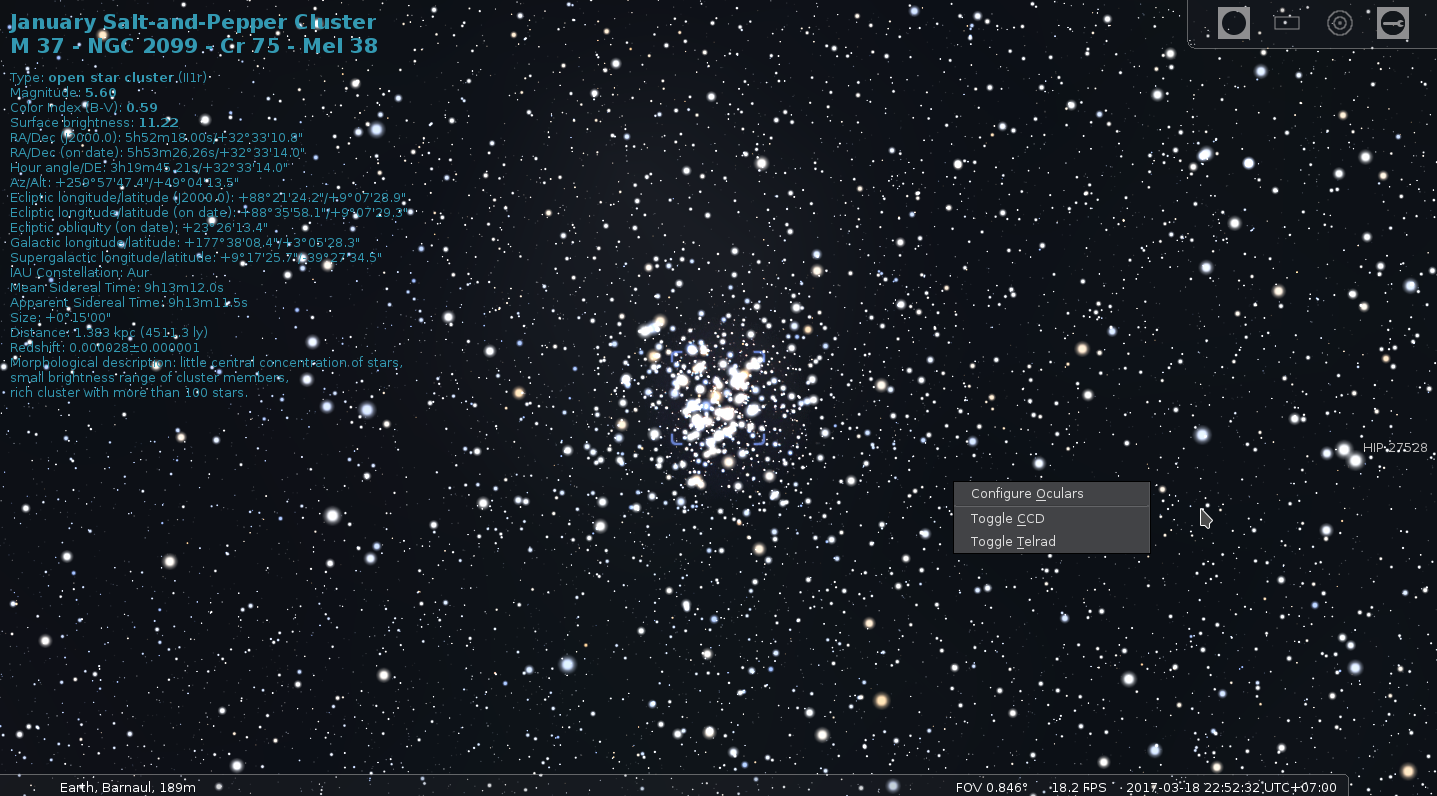
\includegraphics[width=.75\textwidth]{oculars_usage_menu}
\caption{The on-screen menu (top right) and popup menu (lower right) of the Oculars plugin.}
\label{fig:plugins:Oculars:Usage:Menu}
\end{figure}

The options available in the popup menu depend on what you are currently doing. 
In the default menu, you can choose to configure the plugin, activate a CCD, or activate the Telrad finder (see fig.~\ref{fig:plugins:Oculars:Usage:Menu}).
The menu is navigated by either the arrow keys on your keyboard or by your mouse. 
The \keys{\arrowkeyup} and \keys{\arrowkeydown} arrow keys move the selection up or down the menu, 
and the \keys{\arrowkeyleft} and \keys{\arrowkeyright}  arrow keys display or hide sub-menus. \keys{\return} activates an option.

\paragraph{Telrad Finder}

The Telrad view can be used without defining any of the items below. 
As a reflex sight is non-magnifying, this feature can only be enabled when no eyepiece is selected. 
You still may want to zoom in a bit to better see which stars are in the circles (fig.~\ref{fig:plugins:Oculars:Usage:Telrad}).
The three circles that appear in the center of the screen are $0.5\degree$, $2.0\degree$, and $4.0\degree$ in diameter. 
They stay centered in the screen, so move the ``telescope'' (click-drag the background) to center the circles on the object of interest. 

\begin{figure}[b]\centering
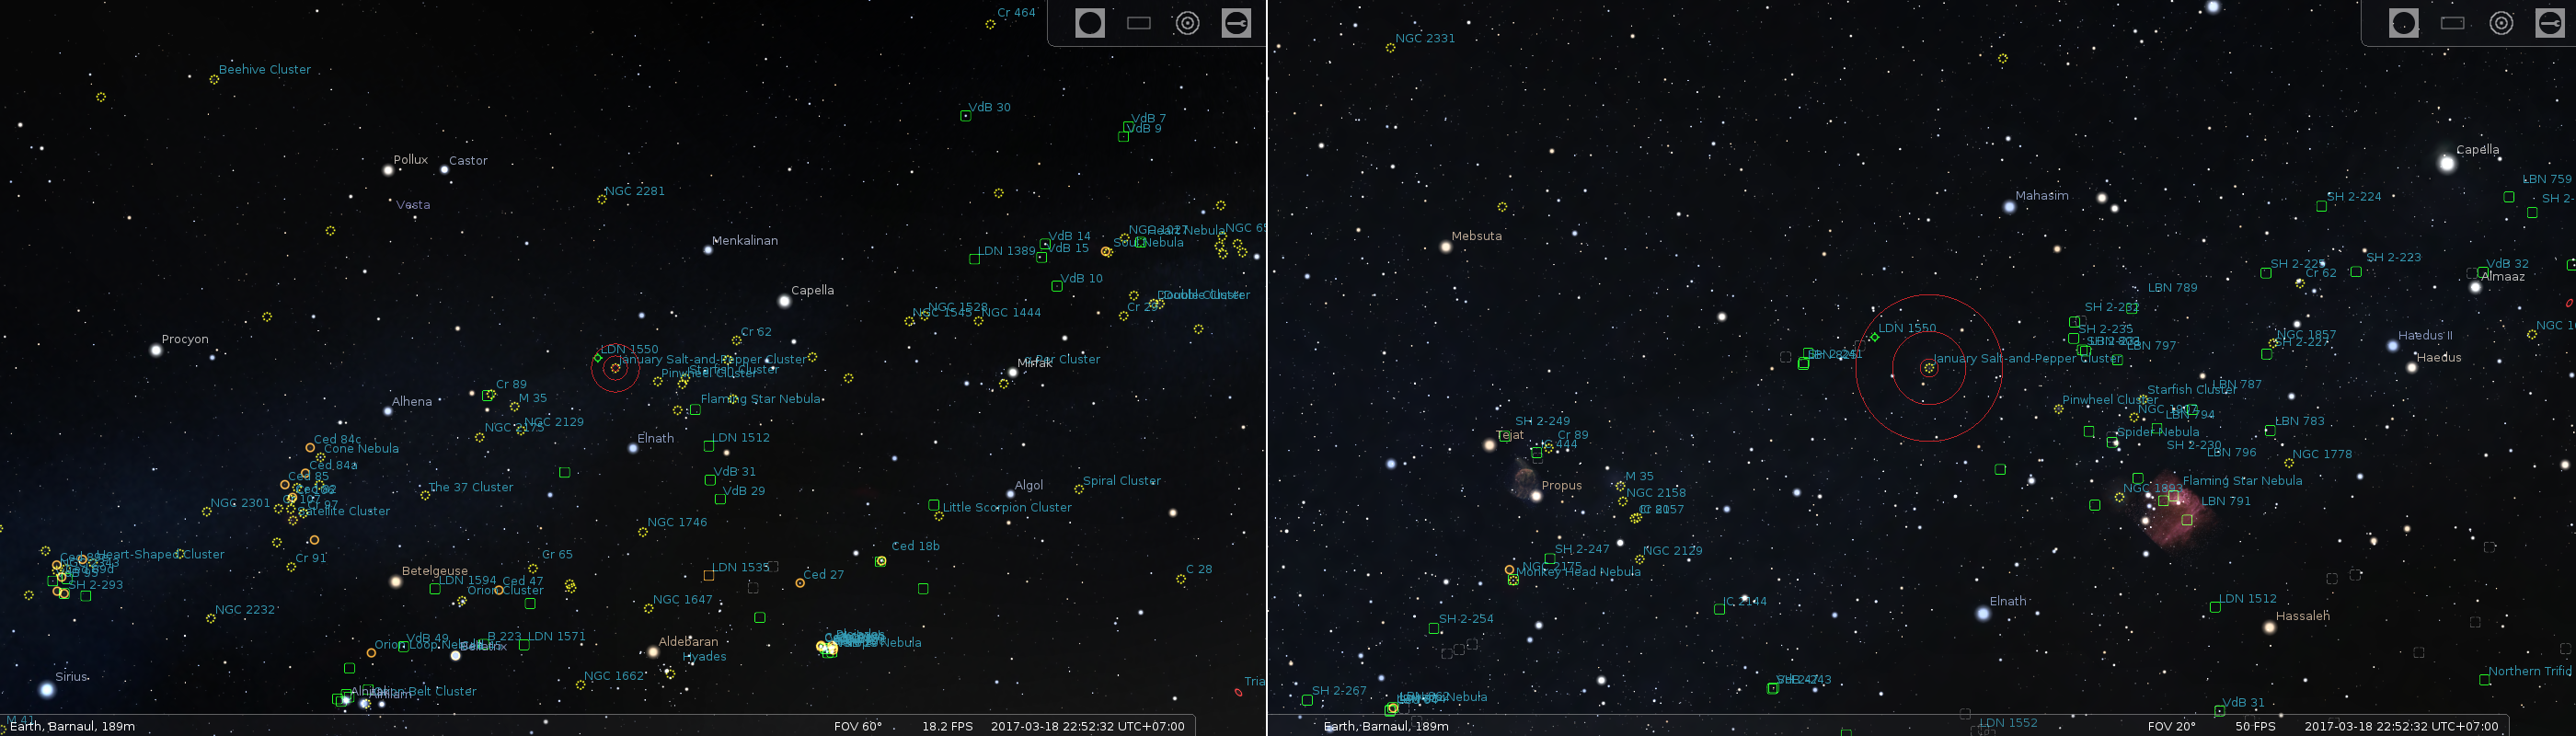
\includegraphics[width=\textwidth]{oculars_usage_telrad}
\caption{The left image is the default $60\degree$, and the right one is $40\degree$.}
\label{fig:plugins:Oculars:Usage:Telrad}
\end{figure}

While the Telrad finder is active, you can not activate a CCD with the popup menu, but only with the on-screen menu.

\paragraph{CCD Sensors}


\begin{figure}[ht]\centering
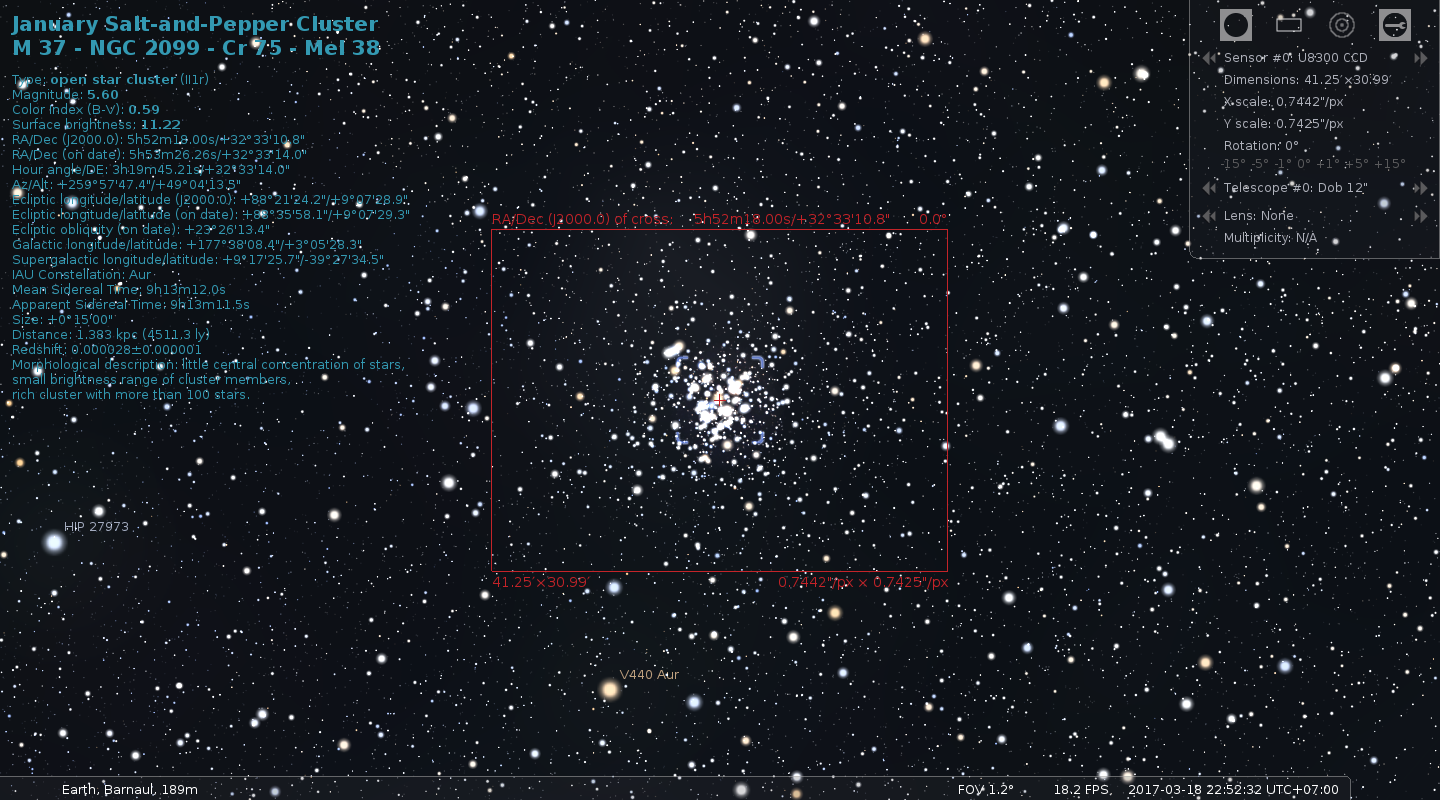
\includegraphics[width=.75\textwidth]{oculars_usage_ccd}
\caption{View of M37 through a CCD sensor of the Oculars plugin.}
\label{fig:plugins:Oculars:Usage:CCD}
\end{figure}

\begin{figure}[ht]\centering
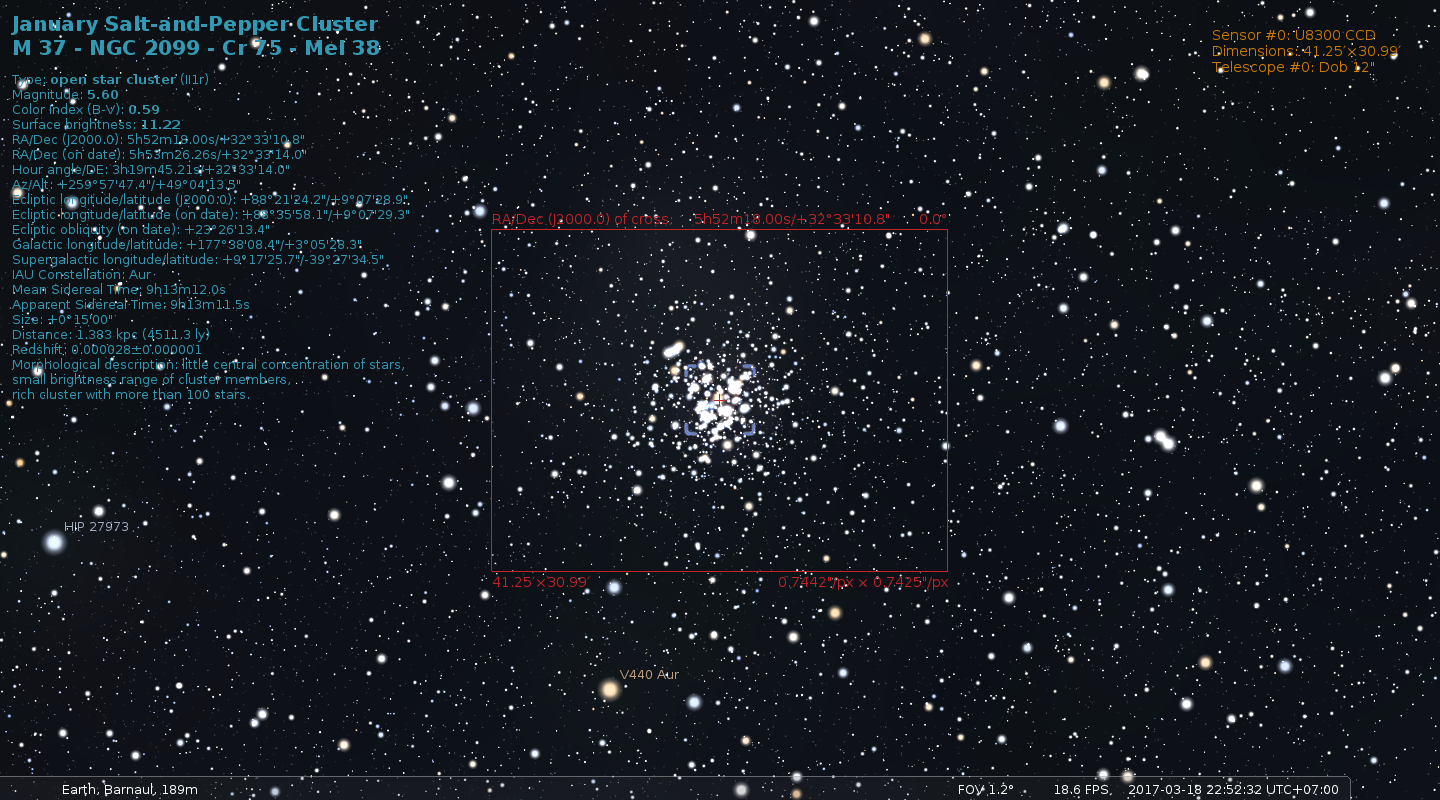
\includegraphics[width=.75\textwidth]{oculars_usage_ccd_info}
\caption{View of M37 through a CCD sensor of the Oculars plugin (without on-screen control panel).}
\label{fig:plugins:Oculars:Usage:CCD:Info}
\end{figure}

\noindent This is a great way to get an idea of what a particular camera will be able to capture when attached to a particular telescope or lens. 
For using camera lenses, you must describe them as telescope with the appropriate values for the lens. 
When active, this feature will display a red bounding box of the area that will be captured, 
as well as zoom in to give a better view of the surroundings. You can manually zoom in or out from there.

The default CCD view will appear similar to fig. \ref{fig:plugins:Oculars:Usage:CCD} or, 
when you are working without the on-screen control panel, the information area in the upper right hand corner 
also shows angular size captured by the CCD (see fig. \ref{fig:plugins:Oculars:Usage:CCD:Info}).


When a CCD view is displayed, the popup menu changes  as seen in  fig. \ref{fig:plugins:Oculars:Usage:CCD:Menu}. 
You can select what telescope to use, as well as progress to the previous or next CCD, or go to a specific CCD. 
You can also rotate the CCD to better frame your subject, or to see if the CCD can be rotated in such a way as to 
catch your area of interest (see fig. \ref{fig:plugins:Oculars:Usage:CCD:RotMenu}). 
Once rotated, the CCD frame on screen displays the new orientation (see fig. \ref{fig:plugins:Oculars:Usage:CCD:Rotation}).

% THESE 3 should always be together on one float page.
\begin{figure}[p]\centering
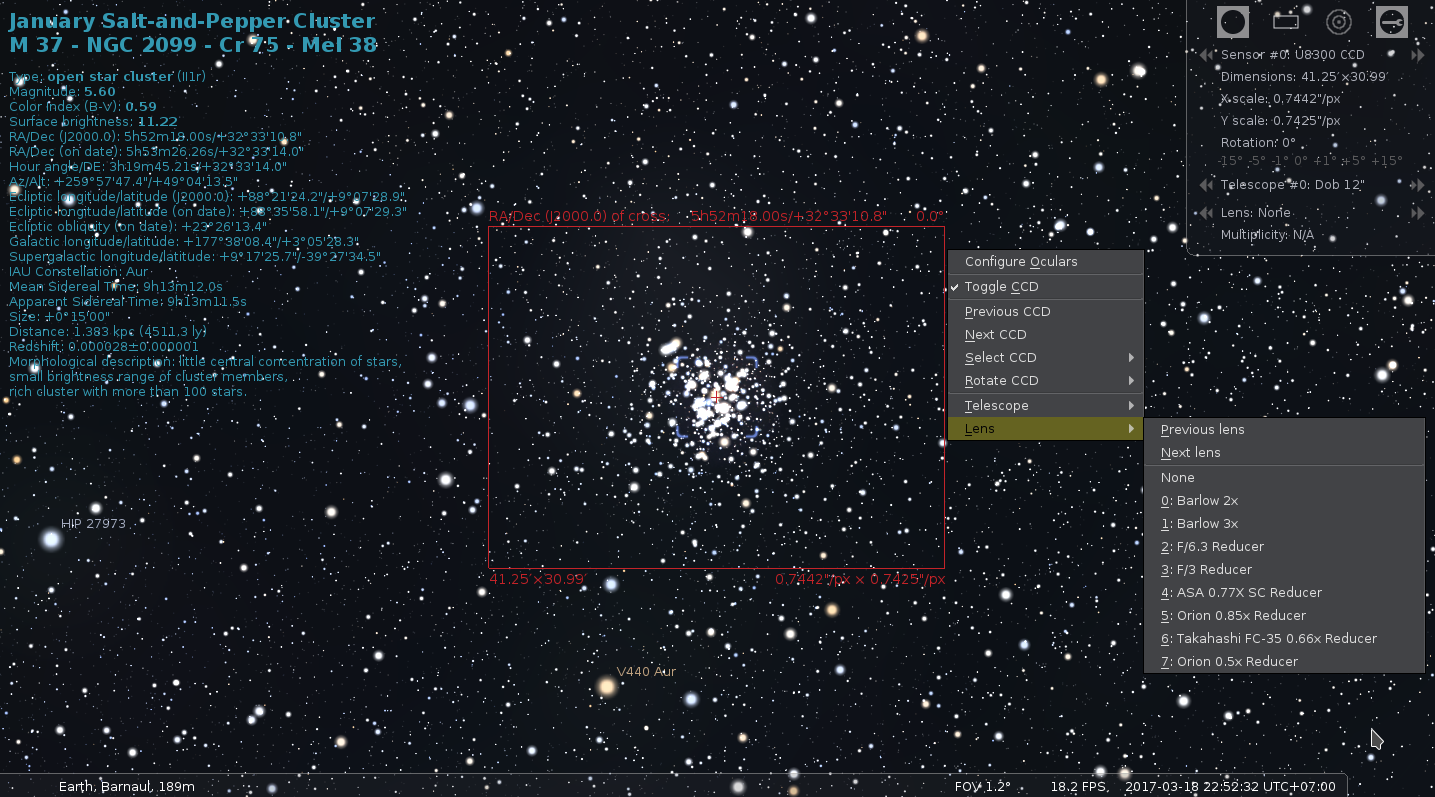
\includegraphics[width=.75\textwidth]{oculars_usage_ccd_menu}
\caption{The CCD sensor popup menu of the Oculars plugin.}
\label{fig:plugins:Oculars:Usage:CCD:Menu}
\end{figure}

\begin{figure}[p]\centering
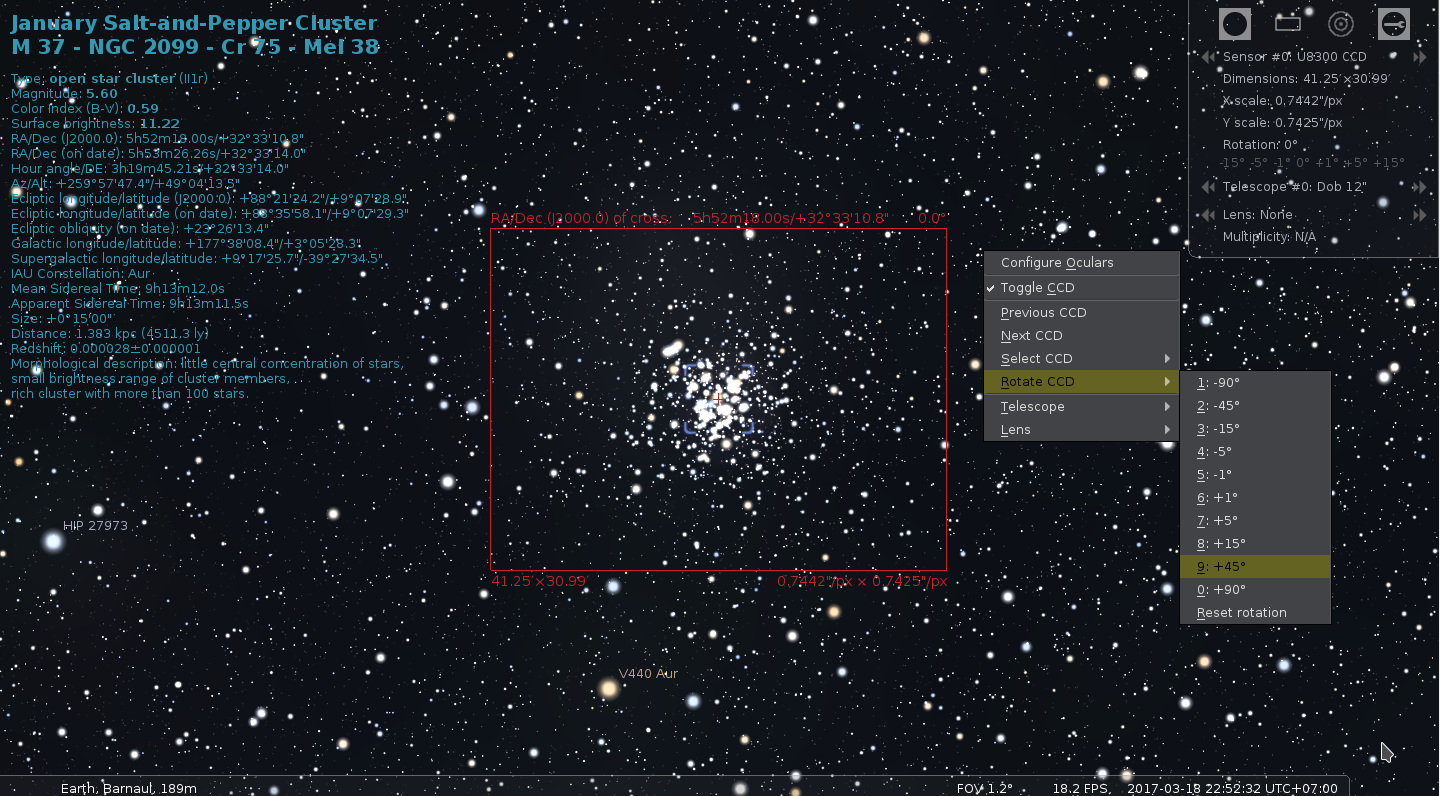
\includegraphics[width=.75\textwidth]{oculars_usage_ccd_rotmenu}
\caption{Setting rotation of CCD sensor in the popup menu.}
\label{fig:plugins:Oculars:Usage:CCD:RotMenu}
\end{figure}

\begin{figure}[p]\centering
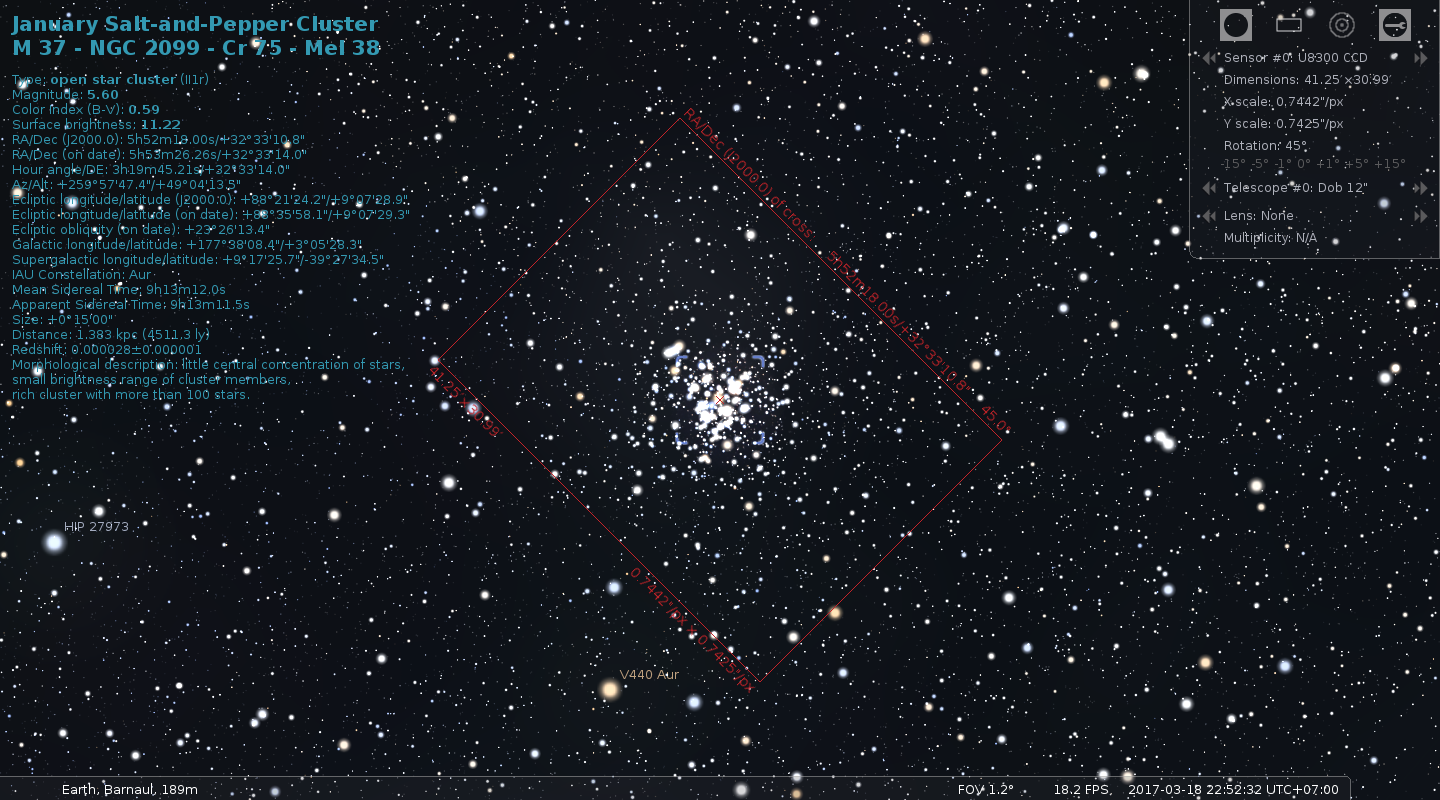
\includegraphics[width=.75\textwidth]{oculars_usage_ccd_rotation}
\caption{A rotated CCD sensor frame of the Oculars plugin.}
\label{fig:plugins:Oculars:Usage:CCD:Rotation}
\end{figure}

\newpage


\paragraph{Oculars}

\begin{itemize}
\item Define some eyepieces and telescope (see section \ref{sec:sec:plugins:Oculars:Configuration}).
\item Select an object to view (i.e. a star, planet, etc.)
\item Click the toolbar button \guibutton{0.6}{bt_ocular} for toggling the Ocular view, or press \keys{\ctrl+O} (\keys{\cmdmac+O} for Mac users).
\item Swap between eye pieces and telescopes to see how the view changes.
\end{itemize}

This is really the area of interest to most telescopic observers. 
It is a great way to compare different eyepiece/telescope combinations, to see how they change the view of the sky. 
And it is easy to do so with binoculars too. 
To show this, let us use the M37 cluster as target. Through a pair of Celestron 15x70 binoculars, it would look like in fig.~\ref{fig:plugins:Oculars:Usage:Ocular:M37Binos}.

\begin{figure}[h]\centering
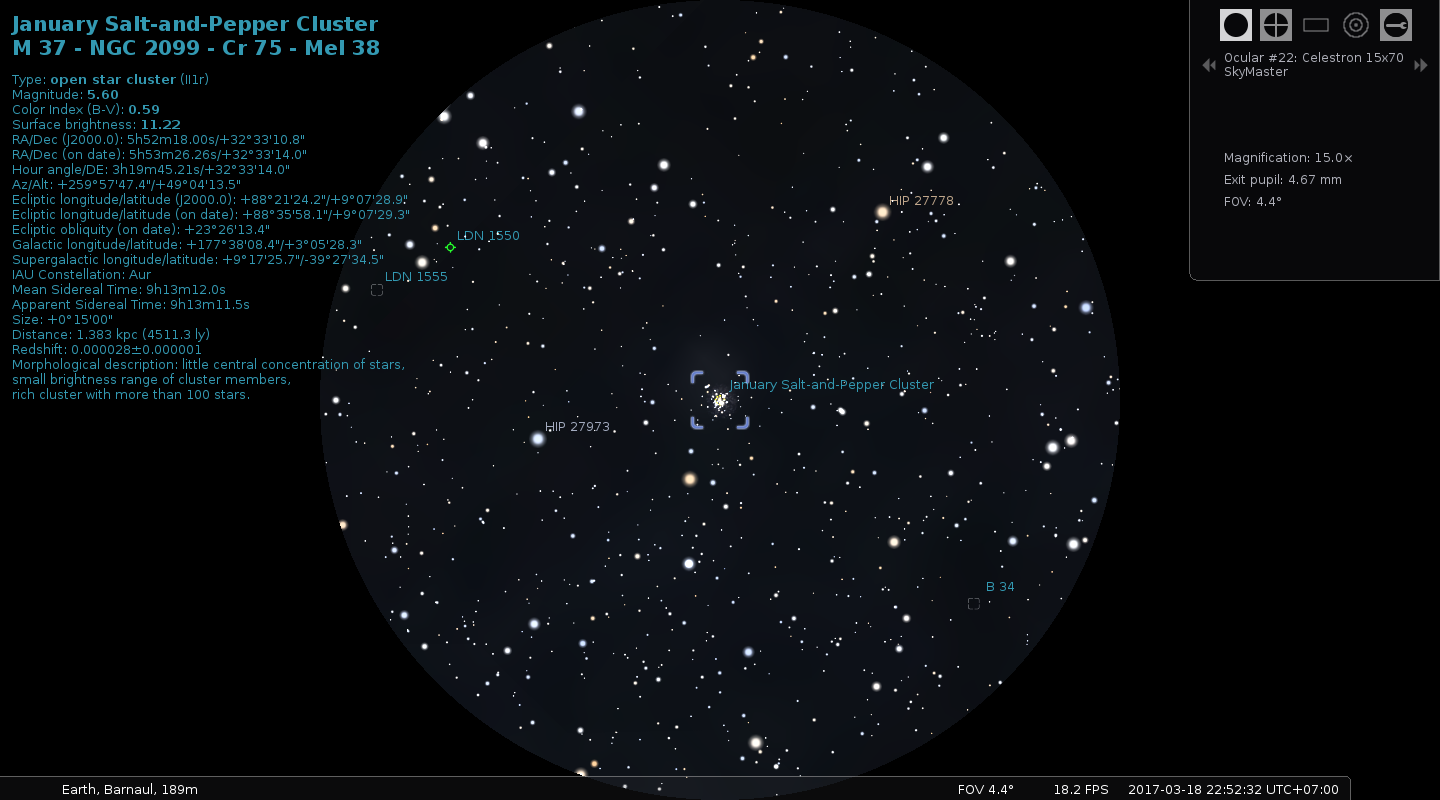
\includegraphics[width=.75\textwidth]{oculars_usage_ocular_m37binos}
\caption{The M37 cluster through a Celestron 15x70 binocular.}
\label{fig:plugins:Oculars:Usage:Ocular:M37Binos}
\end{figure}

\noindent A very pretty sight. Now, what would it look like through a Celestron 80\,mm EDF finder 'scope, with an Explore Scientific 14\,mm $100\degree$ eyepiece? See fig.~\ref{fig:plugins:Oculars:Usage:Ocular:M37EDF}!

\begin{figure}[h]\centering
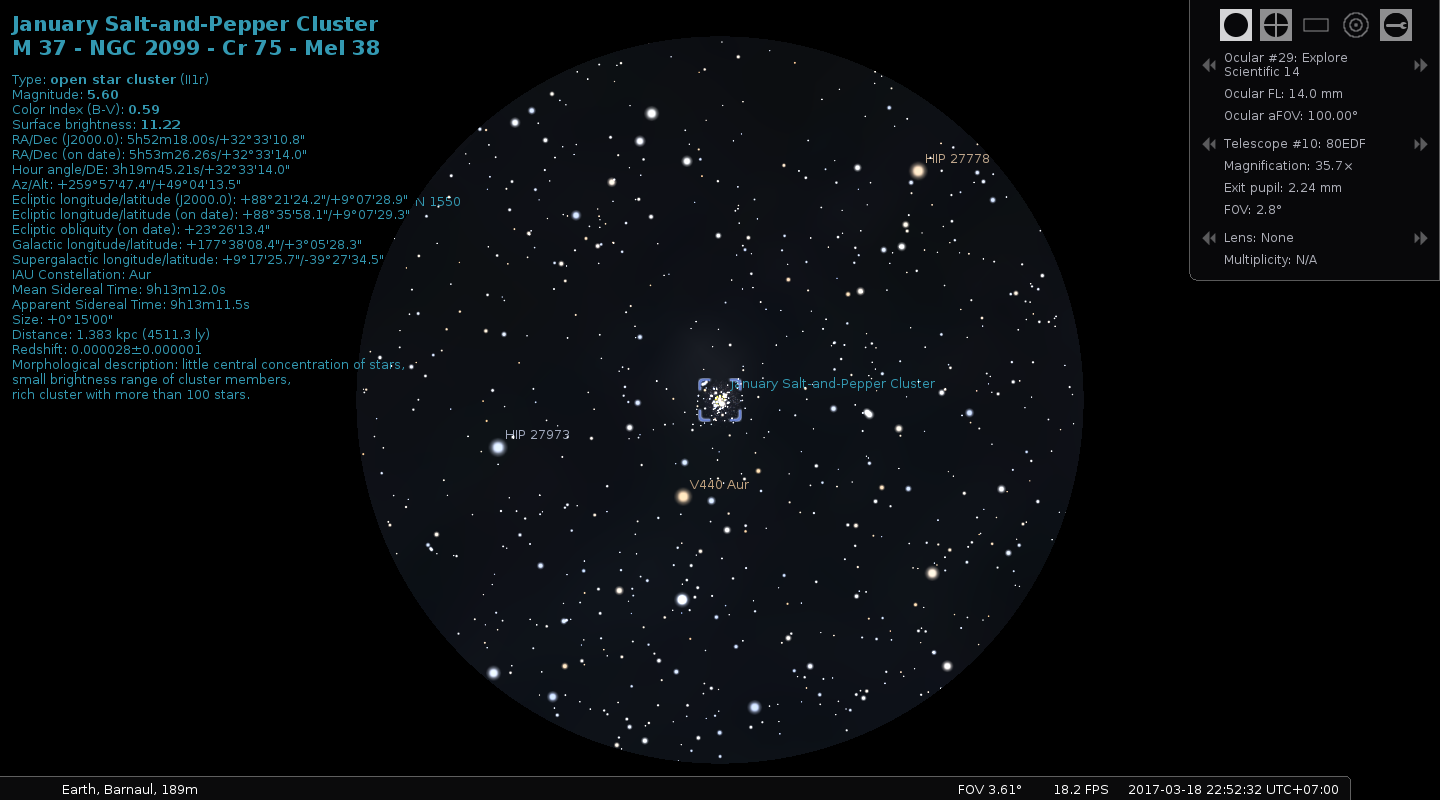
\includegraphics[width=.75\textwidth]{oculars_usage_ocular_m37edf}
\caption{The M37 cluster through a Celestron 80\,mm EDF with Explore Scientific 14\,mm eyepiece.}
\label{fig:plugins:Oculars:Usage:Ocular:M37EDF}
\end{figure}

\noindent Not bad at all. But we like to see more! So we move the eyepiece to a C1400. See fig.~\ref{fig:plugins:Oculars:Usage:Ocular:M37C1400} for the resulting view.

%%%%%%%%%%% MISSING CONTEXT SWITCH!! Here might be a paragraph with comparing the 14mm eyepiece with a 31mm Nagler!

\begin{figure}[ht]\centering
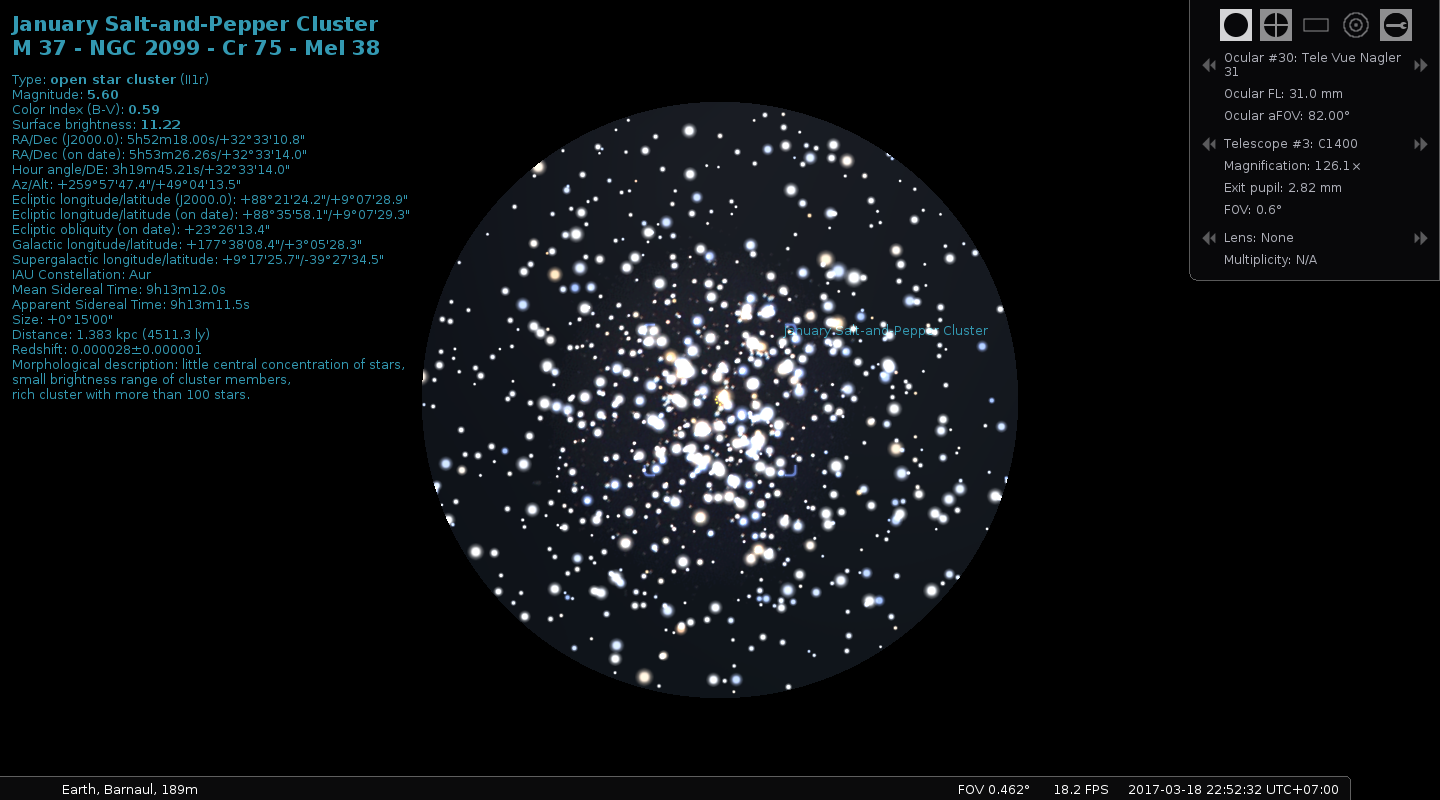
\includegraphics[width=.75\textwidth]{oculars_usage_ocular_m37c1400}
\caption{The M37 cluster through a Celestron C1400 with Tele Vue Nagler 31\,mm eyepiece.}
\label{fig:plugins:Oculars:Usage:Ocular:M37C1400}
\end{figure}

Very nice indeed! So for this target, the C1400 is going to be the best bet. However, if my target was the Pleiades, the C1400 with that eyepiece would not be good -- the 80EDF would do much better!

When an eyepiece is active, the popup menu again changes.  
With a non-binocular eyepiece selected, you also have the ability to select a particular eyepiece or telescope.
When a binocular is active, you can not select a telescope, as it is not relevant. 
Changing the eyepiece to a non-binocular will again allow the telescope to be selected. 
Also notice that when your mouse cursor is very near the right hand border of the screen, the popup menu's sub-menus display to the left, not the right.

\subsubsection{Star Scales}
\newFeature{0.16.0}As you know from section~\ref{sec:gui:view:sky}, the number and relative size of stars of various magnitudes 
can be adjusted to your personal preferences in the view settings window to approximate the appearance of the stars as seen by the naked eye. 
Some observers prefer to have a simulated ocular view with very small, or more, stars, quite different from what Stellarium usually shows. 
The Oculars plugin therefore keeps two additional sets of scaling values for ocular views and CCD views, which are activated 
automatically when you switch to ocular or CCD view, and which are stored immediately and permanently in the plugin's \file{ocular.ini} file.\footnote{%
The appearance of stars may depend on various other factors: telescope type, ocular type, quality of optics, seeing, \ldots 
Such details with all combinations cannot meaningfully be stored, though. These values should allow a rapid toggle on any single night.}

\subsection{Configuration}
\label{sec:sec:plugins:Oculars:Configuration}
All configuration is done through the user interface in the application. 
To open the configuration dialog hit the \keys{\Alt+O} key, 
or click the \button{configure} button on the plugin setup dialog (available in the
\menu{Plugins} tab of Stellarium's Configuration window (opened by 
pressing \keys{F2} or the \guibutton[0.25]{2}{btd_config} button in the left toolbar)), 
or the rightmost button of the on-screen panel (if displayed in the top right corner of screen). 
There are six tabs in the configuration dialog: \emph{General}, \emph{Eyepieces}, \emph{Lenses}, \emph{Sensors}, \emph{Telescopes}, and \emph{About}. The first five are the ones we are interested in here.

\paragraph{General}

The first option allows you to define the general behaviour of the plugin. 
The options are grouped by areas of usage: \emph{Interface}, \emph{Ocular view} and \emph{Sensor view} (see figure \ref{fig:plugins:Oculars:Gui:General}).

\begin{figure}[ht]\centering
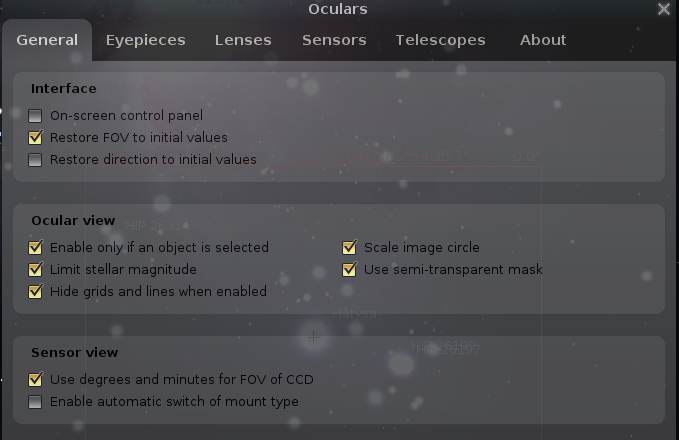
\includegraphics[width=0.75\textwidth]{oculars_gui_general}
\caption{General tab of the Oculars plugin configuration dialog.}
\label{fig:plugins:Oculars:Gui:General}
\end{figure}

\begin{description}
\item[Interface:] this group of options allows to change behaviour of the plugin in general.
 \begin{description}
   \item[On-screen control panel:] show an additional GUI panel in the top-right corner of the screen to allow switching features of the plugin (in addition to the popup window).
   \item[Restore FOV to initial values] and
   \item[Restore direction to initial values] options allow restoration field of view and direction of view, resp., 
         to the initial values at program start at the end of the plugin usage (e.g., when disabling the view through CCD frame).
 \end{description}
\item[Ocular view] is a group of options that allows to change the plugin's behaviour in visual observation mode.
 \begin{description}
   \item[Enable only if an object is selected] -- uncheck this option if you want to use the visual observation mode when no object is selected.
   \item[Limit stellar magnitude] allows to hide faint stars, which are invisible for the selected combination of eyepiece, lens and telescope.
   \item[Hide grids and lines when enabled] allows to hide grids and lines when you observe the sky through the eyepiece and re-enables their visibility when leaving visual observation mode.
   \item[Scale image circle] option allows you to define whether or not to scale the images based on apparent FOV. When deactivated, the image circle will fill your screen. 
         In general, we recommend you not select this, unless you have a need to, because it can really reduce the image size on the screen. 
		 It can however be very useful in comparing two eyepieces. 
		 If you set this option, the  on-screen image will be scaled based on the eyepieces and telescopes you define. 
		 See section \ref{sec:sec:plugins:Oculars:ScalingTheEyepieceView} for information on what scaling means, and why you might want to use it.
   \item[Use semi-transparent mask:] uncheck this option if you want to see visible field of view as in real telescope.
 \end{description}
\item[Sensor view] is group of options allows to change behaviour of the plugin for photographic observations mode.
 \begin{description}
   \item[Use degrees and minutes for FOV of CCD] -- for many cases the use of decimal degrees for the value of the field of view is not comfortable, and this option allows to use the more human readable format for FOV.
   \item[Enable automatic switch of mount type] allows to store the CCD frame orientation when the type of telescope mount is changed.
 \end{description}
\end{description}

\paragraph{Eyepieces}

This is the tab used to enter your own eyepieces (see figures~\ref{fig:plugins:Oculars:Gui:Eyepieces} and \ref{fig:plugins:Oculars:Gui:Eyepieces_binos}). 
By default, a few sample ones have been added; feel free to delete those once you've entered your own.

\begin{figure}[p]\centering
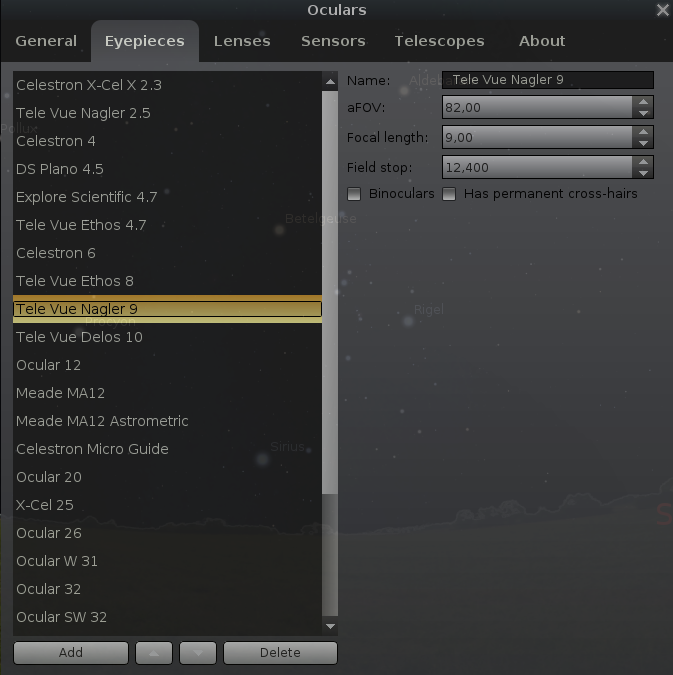
\includegraphics[trim=0 200 0 0,clip,width=.75\textwidth]{oculars_gui_eyepieces}
\caption{Eyepieces tab of Oculars plugin configuration dialog.}
\label{fig:plugins:Oculars:Gui:Eyepieces}
\end{figure}

\begin{figure}[p]\centering
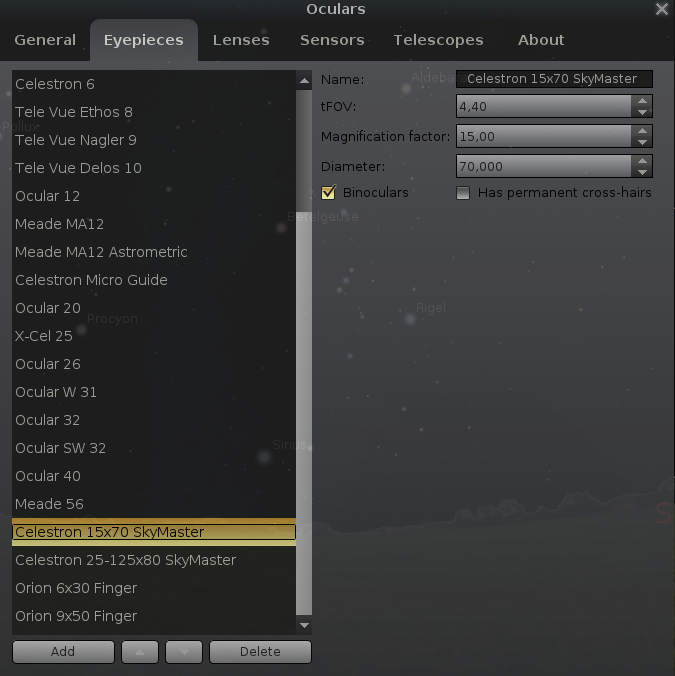
\includegraphics[width=0.75\textwidth]{oculars_gui_eyepieces_binos}
\caption{Eyepieces tab of Oculars plugin configuration dialog (settings for binocular).}
\label{fig:plugins:Oculars:Gui:Eyepieces_binos}
\end{figure}


The fields on this tab are:
\begin{description}
\item[Name] -- a free-text description of the eye piece. You could modify this to match your personal descriptions of eyepieces.
\item[aFOV] -- apparent field of view in degrees.
\item[Focal Length] -- eyepiece focal length in mm.
\item[Field Stop] -- the field stop of the eyepiece in mm. This is used to calculate the true field of view of an eyepiece. If you do not know what it is just leave it the default zero. Not all manufacturers provide this value; TeleVue is one that does.
\item[Binoculars] -- selecting this checkbox tells the system that this eyepiece is binoculars or finders; this means that this eyepiece can be used without defining a telescope.
\item[Has permanent cross-hairs] -- selecting this checkbox tells the system that this eyepiece or binocular (finder) has also simple cross-hairs\footnote{The Oculars plugin supports eyepieces with reticle patterns -- both special eyepieces are available in the default list of eyepieces, and the option \emph{Has permanent cross-hairs} is not related to those eyepieces.}.
\end{description}
When Binoculars are described, the relevant fields change to
\begin{description}
\item[tFOV] -- true field of view in degrees.
\item[Magnification factor] -- the magnification of the binocular.
\item[Diameter] -- the diameter of the binocular objective in mm.
\end{description}


\paragraph{Lenses}

This is the tab used to enter your own lenses (see figure \ref{fig:plugins:Oculars:Gui:Lenses}). By default, a few sample ones have been added; feel free to delete them once you've entered your own.

\begin{figure}[ht]\centering
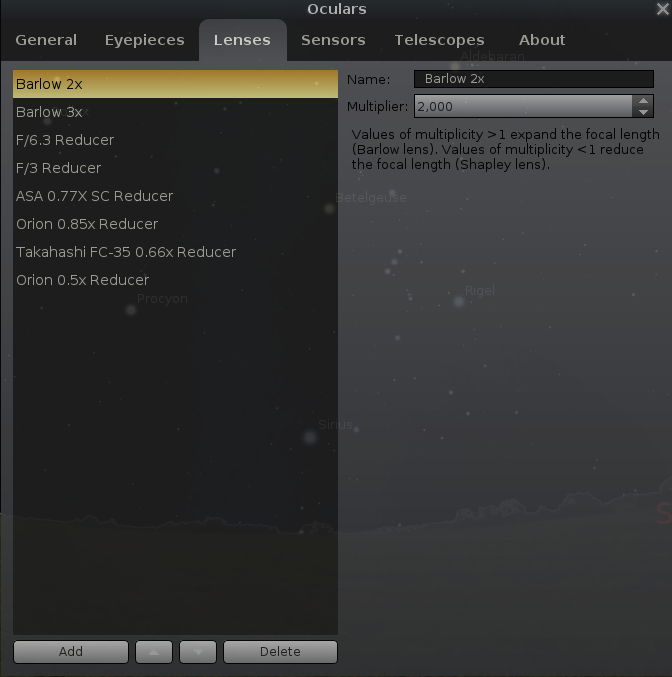
\includegraphics[trim=0 350 0 0,clip,width=.75\textwidth]{oculars_gui_lenses}
\caption{Lenses tab of Oculars plugin configuration dialog.}
\label{fig:plugins:Oculars:Gui:Lenses}
\end{figure}

The fields on this tab are:
\begin{description}
\item[Name] -- a free-text description of the lense. You could modify this to match your personal descriptions of lenses.
\item[Multiplier] -- a factor larger than 1 expands the focal length, and lenses with this type are named Barlow lense; 
                     a factor less   than 1 reduces the focal length, and lenses with this type are named Shapley lense or focus reducer.
\end{description}

\paragraph{Sensors}

This tab allows you to define sensors for any camera you may have (see figure \ref{fig:plugins:Oculars:Gui:Sensors}). 
When defined and selected, this will draw a red bounding rectangle in the center of the eye piece view, showing what the CCD will capture. 
Because of the way floating point numbers are stored, sometimes you may see one of your defined values change (for example from 2.2 to 2.19999) but this should not affect what you see.

\begin{figure}[ht]\centering
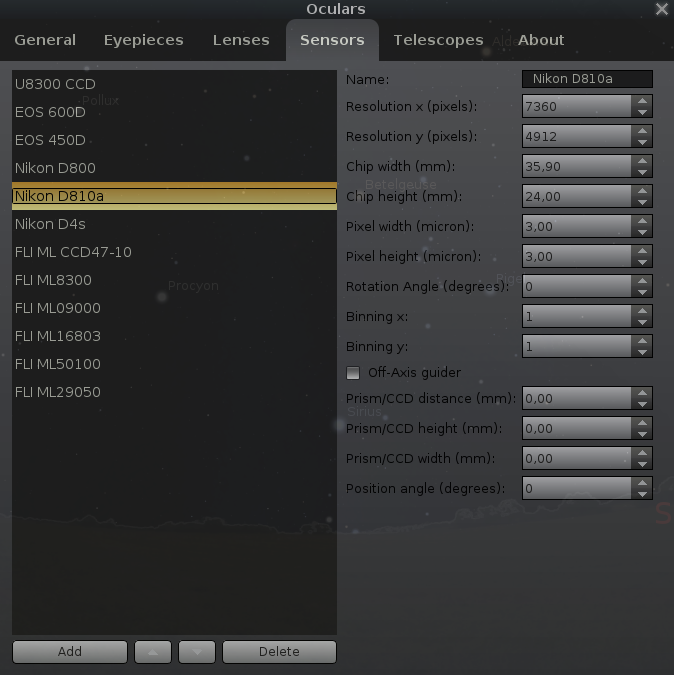
\includegraphics[trim=0 115 0 0,clip,width=.75\textwidth]{oculars_gui_sensors}
\caption{Sensors tab of Oculars plugin configuration dialog.}
\label{fig:plugins:Oculars:Gui:Sensors}
\end{figure}

The fields on this tab are:
\begin{description}
\item[Name] -- A free-text description of the sensor.
\item[Resolution x] -- the width of the sensor in pixels.
\item[Resolution y] -- the height of the sensor in pixels.
\item[Chip width] -- the width of the sensor in mm.
\item[Chip height] -- the height of the sensor in mm.
\item[Pixel width] -- the width of an individual pixel, in \um.
\item[Pixel height] -- the height of an individual pixel, in \um.
\item[Rotation Angle] -- the rotation angle of the sensor, in degrees.
\item[Binning x] -- the binning factor for the width of the sensor.
\item[Binning y] -- the binning factor for the height of the sensor.
\item[Off-Axis guider] -- selecting this checkbox tells the system that this sensor has support an off-axis guider also.
\item[Prism/CCD distance] -- distance between center of prism/CCD of Off-Axis Guider and optical axis of telescope in mm.
\item[Prism/CCD width] -- the width of the prism/CCD of Off-Axis Guider in mm.
\item[Prism/CCD height] -- the height of the prism/CCD of Off-Axis Guider in mm.
\item[Position Angle] -- the position angle of the prism/CCD of Off-Axis Guider, in degrees.
\end{description}

\noindent The resolution is easy to find: these are simply the image dimensions of a (non-binned) frame. 
The chip size and pixel size may be more difficult, but the manual, or searching the Internet, should turn up these values.  
For a ``full-frame'' DSLR, this should be close to 36x24\mm, while APS-C should be around 22.5x15\mm. 
Pixel size is simply image size divided by resolution. Some cameras may have unsquare pixels.

\paragraph{Telescopes}

This is the tab used to enter your own telescopes (see fig.~\ref{fig:plugins:Oculars:Gui:Telescopes}). The fields on this tab are:

\begin{figure}[ht]\centering
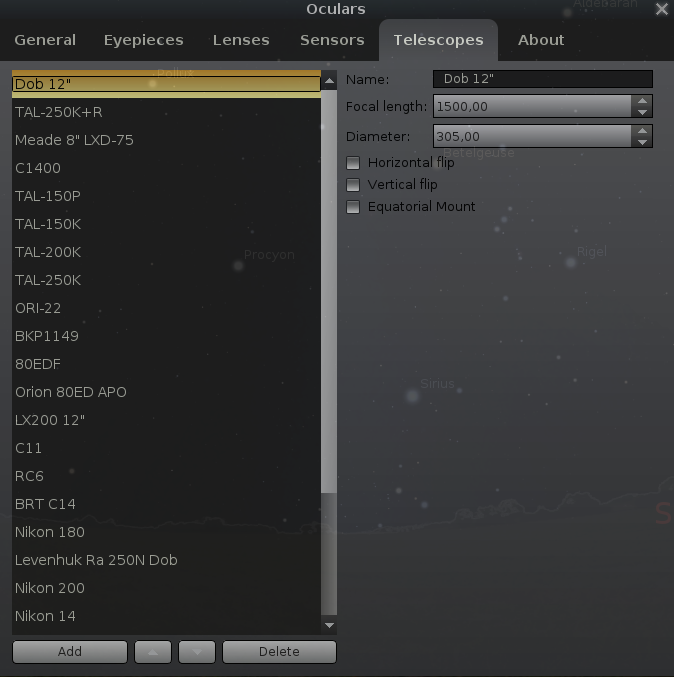
\includegraphics[trim=0 325 0 0,clip,width=.75\textwidth]{oculars_gui_telescopes}
\caption{Telescopes tab of Oculars plugin configuration dialog.}
\label{fig:plugins:Oculars:Gui:Telescopes}
\end{figure}


\begin{description}
\item[Name] -- A free-text description of the telescope. 
\item[Focal Length] -- telescope focal length in mm.
\item[Diameter] -- telescope diameter (aperture) in mm.
\item[Horizontal flip] -- if the view through this telescope should flip horizontally.
\item[Vertical flip] -- if the view through this telescope should flip vertically.
\item[Equatorial Mount] -- select it if this telescope has an equatorial mount.
\end{description}

\subsection{Scaling the eyepiece view}
\label{sec:sec:plugins:Oculars:ScalingTheEyepieceView}
I (TR) would like to thank Al Nagler over at TeleVue\footnote{\url{http://televue.com/}} for helping to set me straight on the topic of eyepieces. They are a lot more complicated than you might think!

By default, the view drawn on your computer screen when the plugin is active fills the screen. That is, there is a circle drawn to represent the view through the eyepiece, and this circle will fill the screen. For general use, this is what most people would want. There will be times that it's not.

If you are going to be observing any deep space object, it can be very important to choose the best eyepiece for that object. You will typically want an eyepiece that will magnify the object as much as possible, while showing all of the object in the eyepiece view. Getting this can be tricky, especially if you do not like changing eyepieces at the telescope. Or maybe you want to understand why one type of telescope may be better than another type for observing what you are interested in. This is where you will want to scale the image on screen based on your eyepiece.

Different eyepieces generally have a different apparent field of view (aFOV). An easy way to think about this is: the larger the aFOV, the bigger the picture you see in the eyepiece. 
Older types of eyepiece (some types still built and in wide use today have been constructed in the 19th century) generally have their aFOV in the $50\degree$ range. 
Today, there are massive eyepieces available with $82\degree$, and recently even $100\degree$ aFOV! 
These eyepieces are huge, as they require a lot of very special glass to achieve their incredible fields of view. 
An eyepiece of the same focal length with a $100\degree$ aFOV will produce an image through the eyepiece that is twice as wide as one produced by a $50\degree$ eyepiece.

Different telescopes, with an eyepiece of a given aFOV, will also produce a different true field of view. 
This is the actual size of the piece of sky that you see through the eyepiece. 
Getting these two ``just right'' can be very important. 
It's easy to assume that you want the biggest telescope you can get, with the eyepiece that gives you the highest magnification. 
This is never true in reality. Depending on where you live, and especially what you like to look at, a 100-120\mm\ quality refractor with a wide aFOV eyepiece may very well be better than a large SCT with the same eyepiece. This is something I learned the hard way.

So how does scaling the eyepiece view help? The plugin will find the eyepiece you have with the largest aFOV. This aFOV becomes $100\%$ of the computer screen diameter. 
Then, any other eyepiece will have its aFOV compared, and the view on screen will be scaled down accordingly. These $100\degree$ aFOV eyepieces makes the math here easy. If you have one, then when that eyepiece is used, the circle that represents the view through the eyepiece will take up $100\%$ of the screen diameter. Next, if you select an eyepiece with an $82\degree$ aFOV, its view will be scaled to $82\%$ of the screen, and a $62\degree$ aFOV eyepiece will be scaled to $62\%$ of the screen.

\paragraph{Example in action}

This is easier to understand in action, so let us look at an example that uses three eyepieces all with the same 17\mm\ focal length, 
so they all produce the same level of magnification (well, one has an 17.3\mm\ focal length, but its magnification is nearly identical) and see how the view changes.
These example all use a Celestron C8 8" SCT telescope, and the target is the Great Orion Nebula.

\begin{figure}[p]\centering
\begin{tabular}{c}
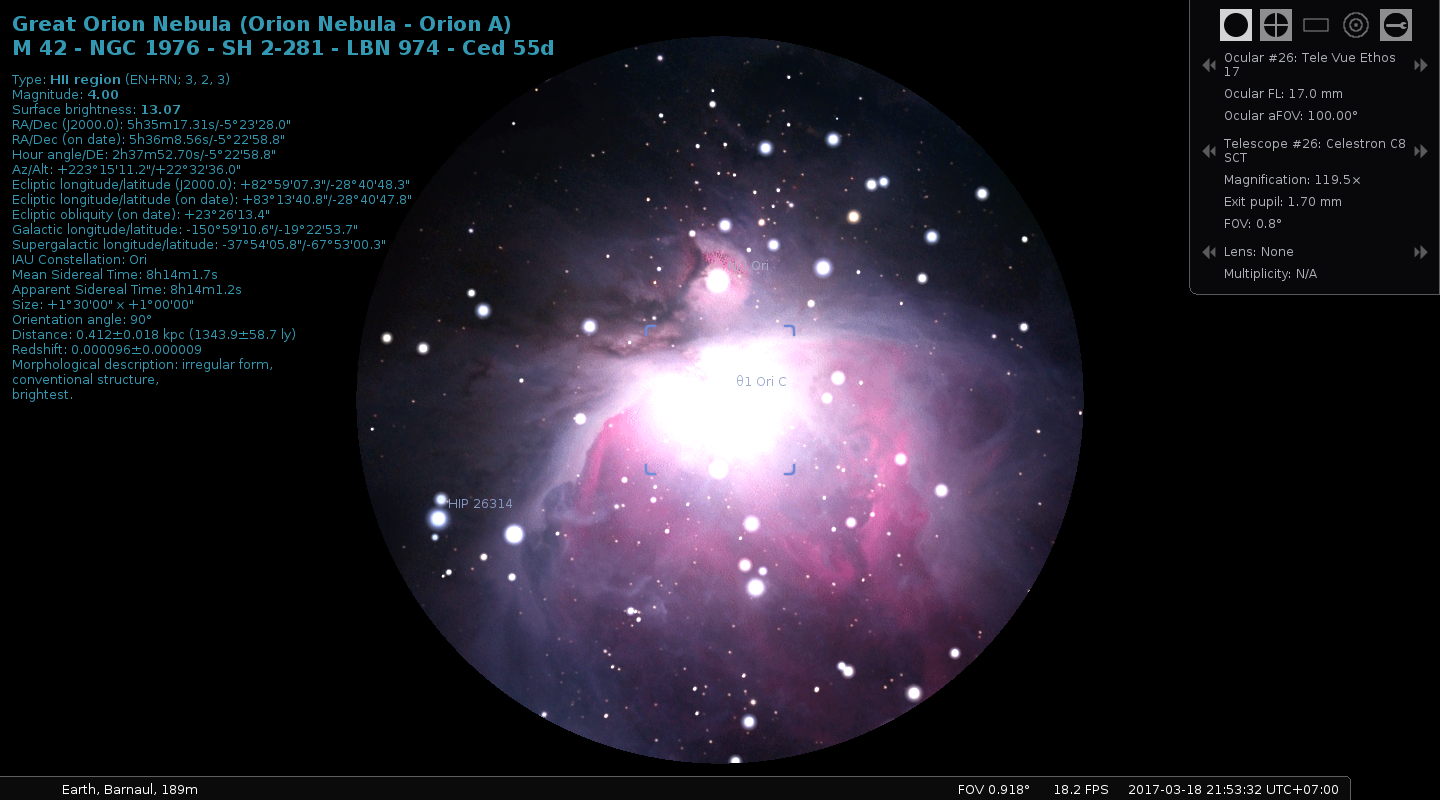
\includegraphics[width=.825\textwidth]{oculars_tv_ethos}\\
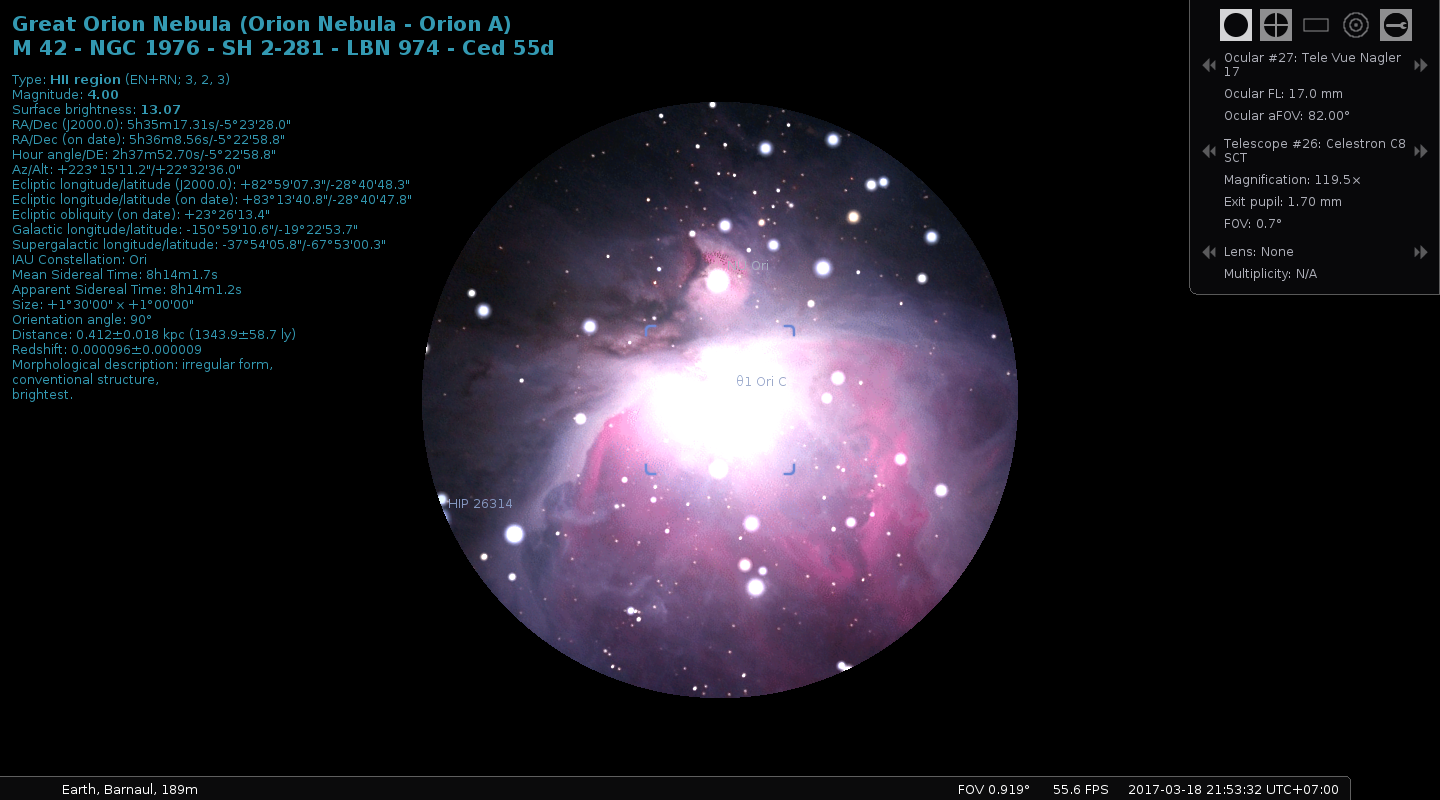
\includegraphics[width=.825\textwidth]{oculars_tv_nagler}\\
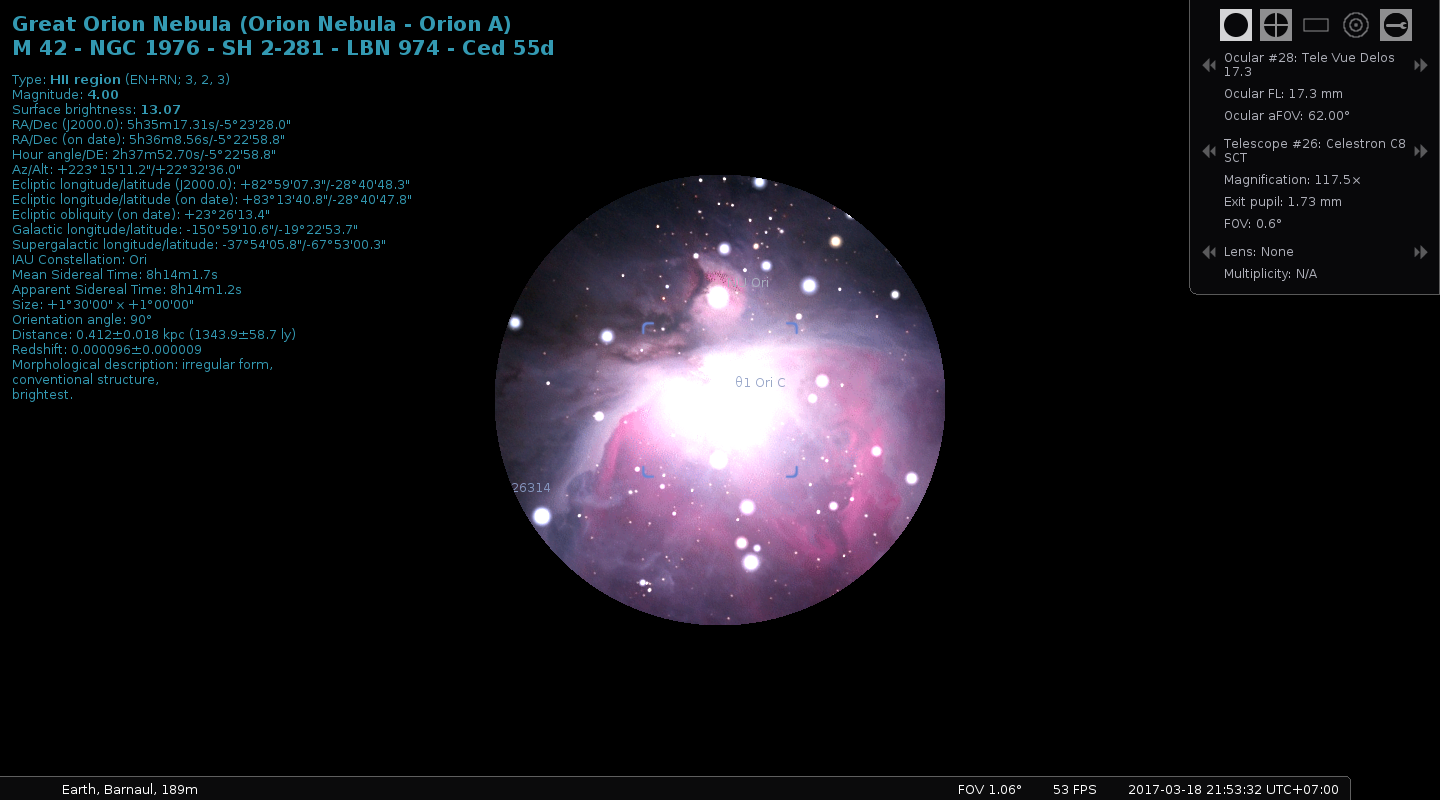
\includegraphics[width=.825\textwidth]{oculars_tv_delos}
\end{tabular}
\caption{Comparing apparent fields of view of (top) a 17\mm\ Tele Vue Ethos eyepiece with an aFOV of $100\degree$. Magnification is $119.5\times$.
(center) a 17\mm\ Tele Vue Nagler eyepiece with an aFOV of $82\degree$. Magnification is $119.5\times$.
(bottom) a 17.3\mm\ Tele Vue Delos eyepiece with an aFOV of $62\degree$. Magnification is $117.5\times$.}
\label{fig:plugins:Oculars:TeleVue}
\end{figure}


We can see from the images in fig.~\ref{fig:plugins:Oculars:TeleVue}
that the target is all three images is the same size. The $100\degree$ image fills the screen, 
the $82\degree$ is smaller, and the $62\degree$ is smallest yet, filling $62\%$ of the computer screen. 
Note that in each image, the field of view that you see changes. The larger the aFOV, the more you can see of the sky. 
So in this example, if you had an 8" telescope, you would want to use the 17\mm\ $100\degree$ Ethos eyepiece to see as much of the nebula as possible.

\newpage
\section{TelescopeControl Plugin}
\label{sec:plugins:TelescopeControl}

This plugin provides a simple control mechanism for motorised
telescope mounts. The user selects an object (i.e.\ by clicking on
something -- a planet, a star etc.) and presses the telescope go-to
key, and the telescope will be guided to the object.

Multiple telescopes may be controlled simultaneously. 

% %TODO Details?
% 
% The control interface uses the Meade or the Celestron protocol and
% most telescopes use either one or the other so many different brands
% of telescopes can be controlled. There is a third party Telescope
% control system going under the name of ASCOM. They provide an
% interface to stellarium and then translate the control into many other
% forms (see section~\ref{sec:plugins:StellariumScope}).
% 
%% GZ Taken from the plugins help page, only slightly reformatted.

\paragraph{WARNING}\emph{Stellarium cannot prevent your
telescope from being pointed at the Sun. It is up to you to ensure
proper filtering and safety measures are applied!}

Never point your telescope at the Sun without a proper solar filter
installed. The powerful light amplified by the telescope WILL cause
\emph{irreversible damage} to your eyes and/or your equipment.

Even if you don't do it deliberately, a slew during daylight hours may
cause your telescope to point at the sun on its way to the given
destination, so it is strongly recommended to avoid using the
telescope control feature before sunset without appropriate
protection.



\subsection{Abilities and limitations}
\label{sec:plugins:TelescopeControl:Limitations}

This plug-in allows Stellarium to send only 'slew' ('go to') commands
to the device and to receive its current position. It cannot issue any
other commands, so users should be aware of the possibility for mount
collisions and similar situations. (To abort a slew, you can start
another one to a safe position.)

Currently this plug-in does not allow satellite tracking unless the controlled 
telescope is an RTS2 system (see section~\ref{sec:plugins:TelescopeControl:RTS2}), 
and is not very suitable for lunar or planetary observations. 
Many mounts can be set to a 'lunar' tracking speed, you may prefer this. 

\subsection{Using this plug-in}
\label{sec:plugins:TelescopeControl:using}

Here are two general ways to control a device with this plug-in, depending on the situation:
\begin{description}
\item[DIRECT CONNECTION] A device supported by the plug-in is
  connected with a cable to the computer running Stellarium

\item[INDIRECT CONNECTION]\mbox{\ } % \\
  \begin{description}
  \item[local] A device is connected to the same computer but it is
    driven by a stand-alone telescope server program or a third-party
    application that can 'talk' to Stellarium;

  \item[remote] A device is connected to a remote computer and the
    software that drives it can 'talk' to Stellarium over the network;
    this software can be either one of Stellarium's stand-alone
    telescope servers, or a third party application.
  \end{description}
\end{description}
Most older telescopes use cables that connect to a serial port
(RS-232), the newer ones use USB (Universal Serial Bus). On Linux and
Max OS X, both cases are handled identically by the plug-in. On
Windows, a USB connection may require a 'virtual serial port'
software, if it is not supplied with the cable or the telescope. Such
a software creates a virtual ('fake') COM port that corresponds to the
real USB port so it can be used by the plug-in. On all three
platforms, if the computer has no 'classic' serial ports and the
telescope can connect only to a serial port, a serial-to-USB
(RS-232-to-USB) adapter may be necessary.

Telescope set-up (setting geographical coordinates, performing
alignment, etc.) should be done before connecting the telescope to
Stellarium.

\subsection{Main window ('Telescopes')}

The plug-in's main window can be opened:
\begin{itemize}
\item By pressing the \button{configure} button for the plug-in in the
  \menu{Plugins} tab of Stellarium's Configuration window (opened by
  pressing \keys{F2} or the \guibutton[0.35]{2}{btd_config} button in the left toolbar).
\item By pressing the \button{Configure telescopes...} button in the \menu{Slew to}
  window (opened by pressing \keys{\ctrl+0} or the respective button on the
  bottom toolbar).
\end{itemize}

\noindent The \menu{Telescopes} tab displays a list of the telescope connections that have been set up:

\begin{itemize}
\item The \emph{number (\#)} column shows the number used to control this
  telescope. For example, for telescope \#2, the shortcut is
  \keys{\ctrl+2}.
\item The \emph{Status} column indicates if this connection is
  currently active or not. Unfortunately, there are some cases in
  which 'Connected' is displayed when no working connection exists.
\item The \emph{Type} field indicates what kind of connection is this:
  \begin{description}
  \item[virtual] means a virtual telescope
  \item[local, Stellarium] means a
    DIRECT connection to the telescope (see above)
  \item[local, external] means an INDIRECT connection to a program
    running on the same computer
  \item[remote, unknown] means an INDIRECT connection over a network
    to a remote machine.
  \end{description}
\end{itemize}

\noindent To set up a new telescope connection, press the \button{Add} button. To modify
the configuration of an existing connection, select it in the list and
press the \button{Configure} button. In both cases, a telescope connection
configuration window will open.



\subsection{Telescope configuration window}

\paragraph{Connection type}
The topmost field represents the choice between the types of connections (see section~\ref{sec:plugins:TelescopeControl:using}):
Telescope controlled by:
\begin{description}
\item[Stellarium, directly through a serial port] is the DIRECT case
\item[External software or a remote computer] is an INDIRECT case
\item[RTS2 Telescope] is another INDIRECT case
\item[Nothing, just simulate one (a moving reticle)] is a \emph{virtual telescope} (no connection)
\end{description}

\paragraph{Telescope properties}

\begin{description}
\item[Name] is the label that will be displayed on the screen next to
  the telescope reticle.
\item[Connection delay] If the movement of the telescope reticle on
  the screen is uneven, you can try increasing or decreasing this
  value.
\item[Coordinate system] Some Celestron telescopes have had their
  firmware updated and now interpret the coordinates they receive as
  coordinates that use the equinox of the date (EOD, also known as
  JNow), making necessary this setting.
\item[Start/connect at startup] Check this option if you want
  Stellarium to attempt to connect to the telescope immediately after
  it starts. Otherwise, to start the telescope, you need to open the
  main window, select that telescope and press the \button{Start/Connect}
  button.
\end{description}

\paragraph{Device settings}
This section is active only for DIRECT connections (see above).

\begin{description}
\item[Serial port] sets the serial port used by the telescope.  There
  is a pop-up box that suggests some default values:
  \begin{itemize}
  \item On Windows, serial ports \texttt{COM1} to \texttt{COM10}
  \item On Linux, serial ports \texttt{/dev/ttyS0} to
    \texttt{/dev/ttyS3} and USB ports \texttt{/dev/ttyUSB0} to
    \texttt{/dev/ttyUSB3}. Make sure you have read/write access to the \texttt{tty} device. 
	Depending on your flavour of Linux, this may e.g.\ require some group membership.
  \item On Mac OS X, the list is empty as it names its ports in a
    peculiar way.
  If you are using an USB cable, the default serial port of your
  telescope most probably is not in the list of suggestions.  To list
  all valid serial port names in Mac OS X, open a terminal and type:

\begin{commands}
  ls /dev/*
\end{commands}
%
This will list all devices, the full name of your serial port should
be somewhere in the list (for example,
\texttt{/dev/cu.usbserial-FTDFZVMK}).
\end{itemize}

\item[Device model]: see~\ref{sec:plugins:TelescopeControl:supported} Supported devices.
\end{description}

\paragraph{Connection settings}
Both fields here refer to INDIRECT connections, which implies communication over a network (TCP/IP). 
\begin{description}
\item[Host] can be either a host name or an IPv4 address such as
  '127.0.0.1'.  The default value of 'localhost' means 'this
  computer'. 

  Modifying the default host name value makes sense only if you are
  attempting a remote connection over a network. In this case, it
  should be the name or IP address of the computer that runs a program
  that runs the telescope.
\item[Port] refers to the TCP port used for communication. The default
  value depends on the telescope number and ranges between 10001 and
  10009.
\end{description}

\paragraph{RTS2 settings} (see also \ref{sec:plugins:TelescopeControl:RTS2})
You will need access to RTS2 HTTPD server through HTTP/JSON calls. Please see
RTS2 documentation (man rts2-httpd) for details. You will as well need username
and password for HTTPD. Please be aware that in order to move the telescope,
your user must have the telescope in the list of allowed devices in the database. Please see \texttt{man
rts2-user} for details on how to manipulate RTS2 users.

\begin{description}
\item[URL] points to RTS2 HTTPD. Can include anything a URL can have - port
  (:8889) and prefix path for RTS2 access.
\item[Username] username used for login to RTS2 HTTPD.
\item[Password] password for login to RTS2 HTTPD.
\end{description}

\paragraph{User Interface Settings: Field of view indicators}

A series of circles representing different fields of view can be added
around the telescope marker. This is a relic from the times before the
Oculars plug-in (see~\ref{sec:plugins:Oculars}) existed.

Activate the 'Use field of view indicators' option, then enter
a list of values separated with commas in the field below. The values
are interpreted as degrees of arc.

These marks can be used in combination with a virtual telescope to
display a moving reticle with the Telrad circles.


\subsubsection{'Slew telescope to' window}

The \menu{Slew telescope to} window can be opened by pressing \keys{\ctrl+0} or the respective button in the bottom toolbar.

It contains two fields for entering celestial coordinates, selectors
for the preferred format (Hours-Minutes-Seconds,
Degrees-Minutes-Seconds, or Decimal degrees), a drop-down list and two
buttons.

The drop-down list contains the names of the currently connected
devices. If no devices are connected, it will remain empty, and the
\button{Slew} button will be disabled.

Pressing the \button{Slew} button slews the selected device to the selected set
of coordinates. See the section about keyboard commands below for
other ways of controlling the device.

Pressing the \button{Configure telescopes\ldots} button opens the main window of
the plug-in.

TIP: Inside the 'Slew' window, underlined letters indicate that
pressing \keys{\Alt + underlined letter} can be used instead of
clicking. For example, pressing \keys{\Alt+S} is equivalent to
clicking the \button{Slew} button, pressing \keys{\Alt+E} switches to
decimal degree format, etc.


\subsubsection{Sending commands}

Once a telescope is successfully started/connected, Stellarium
displays a telescope reticle labelled with the telescope's name on its
current position in the sky. The reticle is an object like every other
in Stellarium - it can be selected with the mouse, it can be tracked
and it appears as an object in the 'Search' window.

To point a device to an object: Select an object (e.g. a star) and
press the number of the device while holding down the \keys{\ctrl} key. (For
example, \keys{\ctrl+1} for telescope \#1.) This will move the telescope to the
selected object. Note that most telescopes can only execute a single command to 
move to that object's position, but if the telescope is an RTS2 telescope, 
you can even track a satellite (if the mount then is fast enough to support it).%
\footnote{Actually, the TLE orbital elements of the selected satellite are transmitted 
to RTS2, which does then compute the satellite position itself.}

To point a device to the center of the view: Press the number of the
device while holding down the Alt key. (For example, \keys{\Alt+1} for
telescope \#1.) This will slew the device to the point in the center of
the current view. (If you move the view after issuing the command, the
target won't change unless you issue another command.)

To point a device to a given set of coordinates: Use the \menu{Slew to} window (press \keys{\ctrl+0}).

\subsection{Supported devices}
\label{sec:plugins:TelescopeControl:supported}

\subsubsection{Directly connected telescopes}
All devices listed in the 'Device model' list are convenience
definitions using one of the two built-in interfaces: the Meade LX200
(the Meade Autostar controller) interface and the Celestron NexStar
interface.

The device list contains the following:
\begin{description}
\item[Celestron NexStar (compatible)] Any device using the NexStar
  interface.
\item[Losmandy G-11] A computerized telescope mount made by Losmandy
  (Meade LX-200/Autostar interface).
\item[Meade Autostar compatible] Any device using the LX-200/Autostar
  interface.
\item[Meade ETX-70 (\#494 Autostar, \#506 CCS)] The Meade ETX-70
  telescope with the \#494 Autostar controller and the \#506 Connector
  Cable Set. According to the tester, it is a bit slow, so its default
  setting of 'Connection delay' is 1.5 seconds instead of 0.5 seconds.
\item[Meade LX200 (compatible)] Any device using the LX-200/Autostar
  interface.
\item[Sky-Watcher SynScan AZ mount] The Sky-Watcher SynScan AZ GoTo
  mount is used in a number of telescopes.
\item[Sky-Watcher SynScan (version 3 or later)] SynScan is also the
  name of the hand controller used in other Sky-Watcher GoTo mounts,
  and it seems that any mount that uses a SynScan controller version
  3.0 or greater is supported by the plug-in, as it uses the NexStar
  protocol.
\item[Wildcard Innovations Argo Navis (Meade mode)] Argo Navis is a
  'Digital Telescope Computer' by Wildcard Innovations. It is an
  advanced digital setting circle that turns an ordinary telescope
  (for example, a dobsonian) into a 'Push To'' telescope (a telescope
  that uses a computer to find targets and human power to move the
  telescope itself). Just don't forget to set it to Meade
  compatibility mode and set the baud rate to 9600B1.
\end{description}

\subsubsection{RTS2 telescopes}
Setting up a robotic telescope and dome control system with RTS2 
is beyond the scope of this handbook, but see section~\ref{sec:plugins:TelescopeControl:RTS2} 
for a few notes to be able to connect and command the telescope with Stellarium.
Please refer to the RTS2 Web pages\footnote{\url{http://rts2.org/}} for further details.

Please be aware that some RTS2 usernames might have only read-only access. If this is
case for your username, the telescope marker will be painted red (or
\texttt{color\_telescope\_readonly} from Stellarium's settings file).

\subsubsection{Virtual telescope}
If you want to test this plug-in without an actual device connected to
the computer, choose ``Nothing, just simulate one (a moving reticle)'' in
the \menu{Telescope controlled by:} field. It will show a telescope reticle
that will react in the same way as the reticle of a real telescope
controlled by the plug-in.  See the section above about field of view
indicators for a possible practical application (emulating 'Telrad'
circles).  

%% We don't neeed this remark any longer after 5 years...
%This feature is equivalent to the 'Dummy' type of telescope
%supported by Stellarium's original telescope control feature.


\section{RTS2}
\label{sec:plugins:TelescopeControl:RTS2}

\indexterm{RTS2}, the Remote Telescope System 2, is a complete robotic observatory control system for Linux 
by Petr Kub\'{a}nek, who kindly provided the plugin code to make RTS2 interoperate with Stellarium.
We cannot give a full manual or any further support for RTS2 here, please refer to its website\footnote{\url{http://rts2.org}} 
for complete instructions about dome control, cameras, filter wheels, weather sensors, etc. 
A few notes may be useful for beginners, though. 

RTS2's central piece is a daemon. Start the system:
\begin{commands}
sudo service rts2 start
\end{commands}
RTS2's main control screen is text-based, \program{rts2-mon}. For a quick check, switch on the system using \key{F9}. 
Telescope \texttt{T0} is a dummy telescope which you can select and operate with commands like \texttt{move 120 35} 
(this moves to RA=120°=8h, DEC=35°, but only when this position is above your horizon).

Stellarium's Telescope plugin can communicate with RTS2 using the RTS2 web interface. You must run \program{rts2-httpd} for this, 
which may require the right permissions to write the lock files in \file{/var/run}. This program requires 
that a database has been created as described in the file \file{RUN} in RTS2's source directory and on the RTS2 website\footnote{\url{http://rts2.org/faq.html}}.   
Also, you must create a 'user' for RTS2. This is not a regular Linux account, but an entry in the RTS2 database. 
Create a user with \program{rts2-user -a <user>}. You should use a password different from your regular Linux password, 
as this will be transmitted in plain text between the computer running Stellarium and the RTS2 control computer, 
and may also be written into Stellarium's logfile. Then you can enable device control for the respective user. 
If you want to send slew commands from Stellarium, make sure to allow access to telescope \texttt{T0}. 
If not, Stellarium will be able to show the telescope marker, but you will not be able to control the telescope. 
To enable control for existing users in the default \file{stars} database, 
\begin{commands}
psql stars
update users set allowed_devices = '*';
\end{commands}

In case you cannot properly connect to the RTS2 telescope or cannot send slew commands, check Stellarium's logfile \file{log.txt} for some diagnostic messages.

RTS2 is the only type of telescope supported by Stellarium which can autonomously track satellites. 
Tracking accuracy fully depends on Stellarium's TLE satellite elements being up-to-date 
(see section~\ref{sec:plugins:Satellites}) and the accuracy of your RTS2 installation.

\newpage
\section{StellariumScope}
\label{sec:plugins:StellariumScope}
\program{StellariumScope} is a free add-on that enables you to control your telescope with Stellarium. 

\begin{figure}[htp]
\begin{center}
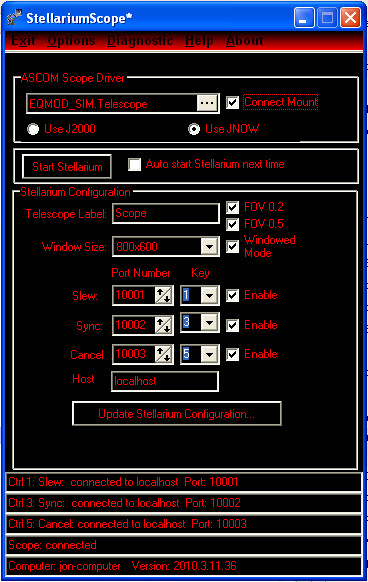
\includegraphics[width=0.85\linewidth]{StellariumScopeFullWindow.jpg}
\end{center}
\caption{\program{StellariumScope} interface}
\label{fig:StellariumScopeFullWindow}
\end{figure}


\paragraph{Features}
\begin{itemize}
\item Provides an interface between Stellarium and ASCOM telescope drivers.
\item Provides the ability to both ``Sync'' and ``Slew'' the
  telescope. It's also possible to issue a stop/cancel command from
  Stellarium.
\item You can easily host Stellarium on one computer linked to another
  control computer that hosts the telescope driver.
\item The installation program will automatically install the
  documentation, but the link to the documentation is provided
  by developer\footnote{\program{StellariumScope} User's Guide --- \url{http://welshdragoncomputing.ca/x/st/misc/stellariumscope_user_guide.2015.10.24.pdf}} so you can read it before installation.
\item There are earlier releases still available on the downloads page on
  Welsh Dragon Computing site.
\end{itemize}

The original \program{StellariumScope} program was designed and implemented by
Scott of ByteArts and is still available for
download\footnote{\url{http://www.bytearts.com/stellarium/}}. If you
have difficulties with the releases available on the Welsh Dragon
Computing
site\footnote{\url{http://welshdragoncomputing.ca/x/index.php/home/stellariumscope/about-stellariumscope}},
you may want to consider using the original version.


Figure~\ref{fig:StellariumScopeFullWindow} shows the interface and
some of the options.  Use this application (like all software that
controls your mount) with supervision of your mount's movements.

\section{Other telescope servers and Stellarium}
\label{sec:plugins:TelescopeControl:Other}

Other developers have also been busy creating hard- and software often
involving Arduino or Raspberry Pi boards which can control GOTO or
PUSHTO (manually driven but position-aware, usually Dobsonian)
telescopes and are ultimately controlled from Stellarium. Those are
not related nor authored by the Stellarium team, so while we welcome
such development (esp.\ open-sourced) in general, we cannot provide
documentation nor any support.

A few examples:
\begin{description}
\item[iTelescope] \url{http://simonbox.info/index.php/astronomy/93-raspberry-pi-itelescope}
\item[node-telescope-server] \url{https://www.npmjs.com/package/node-telescope-server}
\end{description}

One anonymous user sent a troubleshooting solution when connecting Stellarium to the Celestron \program{NexRemote} software:
\begin{quote}
  This involves connecting Stellarium to the \program{NexRemote} software controlling a Celestron NexStar telescope.

  One tricky Window XP issue I fixed was that my older laptop would
  transiently lose connection with Stellarium although the status
  would still be ``Connected'' and all looked normal.

  3 (or whatever) slews would work. Next -- nothing. Although all
  seemed well.

  I boosted the \emph{NexRemote.exe} process in Windows XP to \emph{High} under
  \emph{Set Priority} under the \program{Windows Task Manager} via
  \key{\ctrl+\Alt+Del}.

  All slews now proceed normally. Problem went
  away.\footnote{\url{https://sourceforge.net/p/stellarium/discussion/278769/thread/16e4c054/?limit=25\#8ffa}}
\end{quote}


\newpage
\section{Observability Plugin}
\label{sec:plugins:Observability}

This Plugin  analyzes the observability of the selected object (or the
screen center, if no object is selected). The plugin can show rise,
transit, and set times, as well as the best epoch of the year (i.e.,
largest angular separation from the Sun), the date range when the
source is above the horizon at dark night, and the dates of Acronychal
and Cosmical rise/set.  Ephemerides of the Solar-System objects and
parallax effects are taken into account.

\subsection*{Explanation of some parameters}

\begin{description}
\item[Sun altitude at twilight] Any celestial object will be
  considered visible when the Sun is below this altitude. The altitude
  at astronomical twilight ranges usually between -12 and -18
  degrees. This parameter is only used for the estimate of the range
  of observable epochs (see below).
\item[Horizon altitude] Minimum observable altitude (due to mountains,
  buildings, or just a limited telescope mount).
%% TODO: This should be replaced by the direct interaction with / evaluation of the landscape!!!
\item[Today ephemeris] Self-explanatory. The program will show the
  rise, set, and culmination (transit) times. The exact times for
  these ephemeris are given in two ways: as time spans (referred to
  the current time) and as clock hours (in local time).
\item[Acronychal/Cosmical/Heliacal rise/set] The days of Cosmical
  rise/set of an object are estimated as the days when the object
  rises (or sets) together with the rise/set of the Sun. The exact
  dates of these ephemeris depend on the Observer's location. On the
  contrary, the Acronycal rise (or set) happens when the star
  rises/sets with the setting/rising of the Sun (i.e., opposite to the
  Sun). On the one hand, it is obvious that the source is hardly
  observable (or not observable at all) in the dates between Cosmical
  set and Cosmical rise. On the other hand, the dates around the
  Acronychal set and rise are those when the altitude of the celestial
  object uses to be high when the Sun is well below the horizon (hence
  the object can be well observed). The date of Heliacal rise is the
  first day of the year when a star becomes visible. It happens when
  the star is close to the eastern horizon roughly before the end of
  the astronomical night (i.e., at the astronomical twilight). In the
  following nights, the star will be visibile during longer periods of
  time, until it reaches its Heliacal set (i.e., the last night of the
  year when the star is still visible). At the Heliacal set, the star
  sets roughly after the beginning of the astronomical night.
\item[Largest Sun separation] Happens when the angular separation
  between the Sun and the celestial object are maximum. In most cases,
  this is equivalent to say that the Equatorial longitudes of the Sun
  and the object differ by 180 degrees, so the Sun is in opposition to
  the object. When an object is at its maximum possible angular
  separation from the Sun (no matter if it is a planet or a star), it
  culminates roughly at midnight, and on the darkest possible area of
  the Sky at that declination. Hence, that is the 'best' night to
  observe a particular object.
\item[Nights with source above horizon] The program computes the range
  of dates when the celestial object is above the horizon at least
  during one moment of the night. By 'night', the program considers
  the time span when the Sun altitude is below that of the twilight
  (which can be set by the user; see above). When the objects are
  fixed on the sky (or are exterior planets), the range of observable
  epochs for the current year can have two possible forms: either a
  range from one date to another (e.g., 20 Jan to 15 Sep) or in two
  steps (from 1 Jan to a given date and from another date to 31
  Dec). In the first case, the first date (20 Jan in our example)
  shall be close to the so-called 'Heliacal rise of a star' and the
  second date (15 Sep in our example) shall be close to the 'Heliacal
  set'. In the second case (e.g., a range in the form 1 Jan to 20 May
  and 21 Sep to 31 Dec), the first date (20 May in our example) would
  be close to the Heliacal set and the second one (21 Sep in our
  example) to the Heliacal rise. More exact equations to estimate the
  Heliacal rise/set of stars and planets (which will not depend on the
  mere input of a twilight Sun elevation by the user) will be
  implemented in future versions of this plugin.
\item[Full Moon] When the Moon is selected, the program can compute
  the exact closest dates of the Moon's opposition to the Sun.
\end{description}

\subsection*{Author}
\label{sec:plugins:Observability:author}
This plugin has been contributed by Ivan Marti-Vidal (Onsala Space Observatory)\footnote{\url{mailto:i.martividal@gmail.com}} with some advice by Alexander Wolf and Georg Zotti.




%%% Local Variables: 
%%% mode: latex
%%% TeX-master: "guide"
%%% End: 

